\documentclass[11pt]{article}
\usepackage{cornell-notes}
\usepackage{mathtools}
\usepackage{needspace}
\usepackage{ragged2e}
\usepackage{adjustbox}
\usepackage{tikz}
\usetikzlibrary{arrows.meta,positioning}
\tcbuselibrary{most}
\geometry{letterpaper,margin=0.72in,headheight=15pt}
\setCornellCollection{Calculus Cornell Notes}
\setCornellUnitType{Chapter}
\setCornellUnitNumber{4}
\setCornellUnitTitle{Integration}

\definecolor{Ink}{HTML}{17324D}
\definecolor{Teal}{HTML}{147D78}
\definecolor{Sky}{HTML}{DDEEF1}
\definecolor{Cue}{HTML}{EEF2F5}
\definecolor{Warm}{HTML}{FFF3D6}
\definecolor{Alert}{HTML}{9D3C32}
\definecolor{Green}{HTML}{276749}
\definecolor{Rule}{HTML}{AAB8C2}
\hypersetup{colorlinks=true,linkcolor=Ink,urlcolor=Teal,pdfborder={0 0 0}}
\setlength{\parindent}{0pt}
\setlength{\parskip}{4pt}
\setlist{nosep,leftmargin=*}
\titleformat{\section}{\Large\bfseries\color{Ink}}{}{0pt}{}[\color{Teal}\titlerule]
\titleformat{\subsection}{\large\bfseries\color{Teal}}{}{0pt}{}
\pagestyle{fancy}
\fancyhf{}
\fancyhead[L]{\small\color{Ink}\textsc{Cornell Notes}}
\fancyhead[R]{\small\color{Teal}\nouppercase{\leftmark}}
\fancyfoot[L]{\footnotesize\color{Ink}Active recall $\bullet$ Worked reasoning $\bullet$ Verification}
\fancyfoot[R]{\footnotesize\color{Ink}\thepage\ of \pageref*{LastPage}}
\renewcommand{\headrulewidth}{0.5pt}
\renewcommand{\footrulewidth}{0.4pt}
\newcolumntype{Y}{>{\RaggedRight\arraybackslash}X}
\newtcolorbox{orientationbox}{enhanced,breakable,colback=Sky,colframe=Teal,boxrule=0.7pt,arc=2mm,title=Chapter orientation,fonttitle=\bfseries}
\newtcolorbox{sectionsummarybox}{enhanced,breakable,colback=white,colframe=Teal,boxrule=0.6pt,arc=1.5mm,left=2mm,right=2mm,top=1mm,bottom=1mm,title=Section synthesis,fonttitle=\bfseries\color{Teal}}
\newtcolorbox{warningbox}{enhanced,breakable,colback=Warm,colframe=Alert,boxrule=0.7pt,arc=1.5mm,title=Common error audit,fonttitle=\bfseries}
\newtcolorbox{checkbox}{enhanced,breakable,colback=white,colframe=Green,boxrule=0.7pt,arc=1.5mm,title=Verification habit,fonttitle=\bfseries}
\newcommand{\cornellcuehead}{\rowcolor{Ink}\color{white}\bfseries Cue / recall prompt & \color{white}\bfseries Notes / reasoning \\\endhead}
\newcommand{\cornellcuerow}[2]{\rowcolor{Cue}#1 & #2 \\\addlinespace[3pt]}
% Table-safe: delegates to the shared Cornell formula box (cornell-notes.sty),
% which cannot emit \pagebreak/\noalign inside longtable cells.
\newcommand{\formula}[1]{\CornellFormula[colback=Sky,colframe=Teal]{#1}}

\title{Chapter 4: Integration\\[2mm]\large Cornell Notes}
\author{}
\date{}
\hypersetup{pdftitle={Chapter 4: Integration - Cornell Notes},pdfauthor={},pdfsubject={Calculus study notes},pdfkeywords={calculus, Cornell notes, active recall}}
\begin{document}
\maketitle
\thispagestyle{fancy}
\begin{orientationbox}
Develop the definite integral from accumulation and area, connect it to antiderivatives, and use substitution to reverse the chain rule. These notes follow the complete local section sequence (247--312) and emphasize definitions, governing results, strategy selection, and verifiable reasoning.
\end{orientationbox}

\section{Prerequisite map}
\begin{minipage}[t]{0.42\textwidth}
\textbf{Bring forward}
\begin{itemize}
\item Limits and continuity
\item Derivative rules
\item Summation notation
\item Area formulas
\end{itemize}
\end{minipage}\hfill
\begin{minipage}[t]{0.54\textwidth}
\textbf{Chapter flow}
\begin{center}
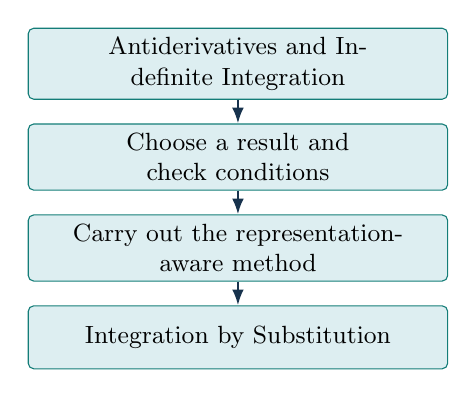
\begin{tikzpicture}[node distance=3mm, every node/.style={font=\small,align=center}, box/.style={draw=Teal,rounded corners=2pt,fill=Sky,minimum height=8mm,text width=0.42\textwidth}, arr/.style={-{Latex[length=2mm]},thick,draw=Ink}]
\node[box] (a) {Antiderivatives and Indefinite Integration};
\node[box,below=of a] (b) {Choose a result and check conditions};
\node[box,below=of b] (c) {Carry out the representation-aware method};
\node[box,below=of c] (d) {Integration by Substitution};
\draw[arr] (a)--(b); \draw[arr] (b)--(c); \draw[arr] (c)--(d);
\end{tikzpicture}
\end{center}
\end{minipage}

\section{Learning objectives}
\begin{enumerate}
\item Explain the central objects and hypotheses in 4.1 and 4.5.
\item Translate among algebraic, graphical, numerical, and verbal representations.
\item Select an appropriate formula or theorem before beginning symbolic work.
\item Carry out multi-step calculations while preserving domain, sign, orientation, and units.
\item Diagnose common errors by testing assumptions and checking the result independently.
\item Synthesize the chapter's methods into a reusable problem-solving workflow.
\end{enumerate}

\section{4.1 Antiderivatives and Indefinite Integration}
\begin{longtable}{C N}\cornellcuehead
\cornellcuerow{What is the governing idea in 4.1?}{An antiderivative reverses differentiation; the indefinite integral represents a family differing by constants.}
\cornellcuerow{Which result should be recalled?}{\formula{\int f(x)\,dx=F(x)+C\quad\text{when }F'=f}}
\cornellcuerow{How should a problem be organized?}{Match the integrand to a derivative rule, integrate term by term where allowed, include $C$, and differentiate the result to verify.}
\cornellcuerow{What should be checked before accepting an answer?}{Confirm the hypotheses and domain, preserve units and orientation when relevant, and substitute or differentiate back into the defining relation.}
\end{longtable}
\begin{warningbox}Omitting the constant loses solutions; distributing powers incorrectly across sums creates false rules.\end{warningbox}
\begin{sectionsummarybox}An antiderivative reverses differentiation; the indefinite integral represents a family differing by constants. The operational habit is to match the integrand to a derivative rule, integrate term by term where allowed, include $C$, and differentiate the result to verify.\end{sectionsummarybox}
\section{4.2 Area}
\begin{longtable}{C N}\cornellcuehead
\cornellcuerow{What is the governing idea in 4.2?}{Area under a curve is approached by sums of rectangle areas whose widths shrink.}
\cornellcuerow{Which result should be recalled?}{\formula{\sum_{i=1}^{n} f(x_i^*)\Delta x}}
\cornellcuerow{How should a problem be organized?}{Partition the interval, choose sample points consistently, form the finite sum, then interpret refinement as a limit.}
\cornellcuerow{What should be checked before accepting an answer?}{Confirm the hypotheses and domain, preserve units and orientation when relevant, and substitute or differentiate back into the defining relation.}
\end{longtable}
\begin{warningbox}Signed height and geometric area differ when the graph lies below the axis.\end{warningbox}
\begin{sectionsummarybox}Area under a curve is approached by sums of rectangle areas whose widths shrink. The operational habit is to partition the interval, choose sample points consistently, form the finite sum, then interpret refinement as a limit.\end{sectionsummarybox}
\section{4.3 Riemann Sums and Definite Integrals}
\begin{longtable}{C N}\cornellcuehead
\cornellcuerow{What is the governing idea in 4.3?}{The definite integral is the limit of Riemann sums and measures signed accumulation over an interval.}
\cornellcuerow{Which result should be recalled?}{\formula{\int_a^b f(x)\,dx=\lim_{\|P\|\to0}\sum f(x_i^*)\Delta x_i}}
\cornellcuerow{How should a problem be organized?}{Check integrability assumptions, preserve bounds and orientation, and use additivity to split complicated intervals.}
\cornellcuerow{What should be checked before accepting an answer?}{Confirm the hypotheses and domain, preserve units and orientation when relevant, and substitute or differentiate back into the defining relation.}
\end{longtable}
\begin{warningbox}Treating a definite integral as automatically positive confuses net change with total area.\end{warningbox}
\begin{sectionsummarybox}The definite integral is the limit of Riemann sums and measures signed accumulation over an interval. The operational habit is to check integrability assumptions, preserve bounds and orientation, and use additivity to split complicated intervals.\end{sectionsummarybox}
\section{4.4 The Fundamental Theorem of Calculus}
\begin{longtable}{C N}\cornellcuehead
\cornellcuerow{What is the governing idea in 4.4?}{The Fundamental Theorem links accumulation functions and antiderivatives, making exact evaluation possible.}
\cornellcuerow{Which result should be recalled?}{\formula{\int_a^b f(x)\,dx=F(b)-F(a),\qquad \frac{d}{dx}\int_a^x f(t)\,dt=f(x)}}
\cornellcuerow{How should a problem be organized?}{Find an antiderivative, evaluate upper minus lower, or combine the accumulation derivative with the Chain Rule for variable bounds.}
\cornellcuerow{What should be checked before accepting an answer?}{Confirm the hypotheses and domain, preserve units and orientation when relevant, and substitute or differentiate back into the defining relation.}
\end{longtable}
\begin{warningbox}Reversing endpoint order or confusing the dummy integration variable with the outer variable changes the result.\end{warningbox}
\begin{sectionsummarybox}The Fundamental Theorem links accumulation functions and antiderivatives, making exact evaluation possible. The operational habit is to find an antiderivative, evaluate upper minus lower, or combine the accumulation derivative with the Chain Rule for variable bounds.\end{sectionsummarybox}
\section{4.5 Integration by Substitution}
\begin{longtable}{C N}\cornellcuehead
\cornellcuerow{What is the governing idea in 4.5?}{Substitution recognizes a composite integrand and reverses the Chain Rule.}
\cornellcuerow{Which result should be recalled?}{\formula{\int f(g(x))g'(x)\,dx=\int f(u)\,du}}
\cornellcuerow{How should a problem be organized?}{Choose $u$ for the inner expression, transform every factor and either change definite bounds or back-substitute, then verify by differentiation.}
\cornellcuerow{What should be checked before accepting an answer?}{Confirm the hypotheses and domain, preserve units and orientation when relevant, and substitute or differentiate back into the defining relation.}
\end{longtable}
\begin{warningbox}Mixing $u$ and $x$ in the same integral or changing bounds and also back-substituting is inconsistent.\end{warningbox}
\begin{sectionsummarybox}Substitution recognizes a composite integrand and reverses the Chain Rule. The operational habit is to choose $u$ for the inner expression, transform every factor and either change definite bounds or back-substitute, then verify by differentiation.\end{sectionsummarybox}

\section{Definitions and theorem register}
\small
\begin{longtable}{@{}>{\RaggedRight\arraybackslash}p{0.24\textwidth}>{\RaggedRight\arraybackslash}p{0.40\textwidth}>{\RaggedRight\arraybackslash}p{0.29\textwidth}@{}}
\toprule
\textbf{Topic} & \textbf{Meaning and conditions} & \textbf{Canonical form}\\
\midrule\endhead
4.1 Antiderivatives and Indefinite Integration & An antiderivative reverses differentiation; the indefinite integral represents a family differing by constants. & \adjustbox{max width=\linewidth}{\(\displaystyle \int f(x)\,dx=F(x)+C\quad\text{when }F'=f\)} \\\addlinespace[2pt]
4.2 Area & Area under a curve is approached by sums of rectangle areas whose widths shrink. & \adjustbox{max width=\linewidth}{\(\displaystyle \sum_{i=1}^{n} f(x_i^*)\Delta x\)} \\\addlinespace[2pt]
4.3 Riemann Sums and Definite Integrals & The definite integral is the limit of Riemann sums and measures signed accumulation over an interval. & \adjustbox{max width=\linewidth}{\(\displaystyle \int_a^b f(x)\,dx=\lim_{\|P\|\to0}\sum f(x_i^*)\Delta x_i\)} \\\addlinespace[2pt]
4.4 The Fundamental Theorem of Calculus & The Fundamental Theorem links accumulation functions and antiderivatives, making exact evaluation possible. & \adjustbox{max width=\linewidth}{\(\displaystyle \int_a^b f(x)\,dx=F(b)-F(a),\qquad \frac{d}{dx}\int_a^x f(t)\,dt=f(x)\)} \\\addlinespace[2pt]
4.5 Integration by Substitution & Substitution recognizes a composite integrand and reverses the Chain Rule. & \adjustbox{max width=\linewidth}{\(\displaystyle \int f(g(x))g'(x)\,dx=\int f(u)\,du\)} \\\addlinespace[2pt]
\bottomrule
\end{longtable}
\normalsize

\section{Formula and method sheet}
\small
\begin{longtable}{@{}>{\RaggedRight\arraybackslash}p{0.08\textwidth}>{\RaggedRight\arraybackslash}p{0.48\textwidth}>{\RaggedRight\arraybackslash}p{0.37\textwidth}@{}}
\toprule
\textbf{Sec.} & \textbf{Method sequence} & \textbf{Stop-and-check trigger}\\
\midrule\endhead
4.1 & Match the integrand to a derivative rule, integrate term by term where allowed, include $C$, and differentiate the result to verify. & Omitting the constant loses solutions; distributing powers incorrectly across sums creates false rules. \\\addlinespace[2pt]
4.2 & Partition the interval, choose sample points consistently, form the finite sum, then interpret refinement as a limit. & Signed height and geometric area differ when the graph lies below the axis. \\\addlinespace[2pt]
4.3 & Check integrability assumptions, preserve bounds and orientation, and use additivity to split complicated intervals. & Treating a definite integral as automatically positive confuses net change with total area. \\\addlinespace[2pt]
4.4 & Find an antiderivative, evaluate upper minus lower, or combine the accumulation derivative with the Chain Rule for variable bounds. & Reversing endpoint order or confusing the dummy integration variable with the outer variable changes the result. \\\addlinespace[2pt]
4.5 & Choose $u$ for the inner expression, transform every factor and either change definite bounds or back-substitute, then verify by differentiation. & Mixing $u$ and $x$ in the same integral or changing bounds and also back-substituting is inconsistent. \\\addlinespace[2pt]
\bottomrule
\end{longtable}
\normalsize

\section{Common errors and diagnostic checks}
\begin{warningbox}
\begin{itemize}
\item \textbf{4.1:} Omitting the constant loses solutions; distributing powers incorrectly across sums creates false rules.
\item \textbf{4.2:} Signed height and geometric area differ when the graph lies below the axis.
\item \textbf{4.3:} Treating a definite integral as automatically positive confuses net change with total area.
\item \textbf{4.4:} Reversing endpoint order or confusing the dummy integration variable with the outer variable changes the result.
\item \textbf{4.5:} Mixing $u$ and $x$ in the same integral or changing bounds and also back-substituting is inconsistent.
\end{itemize}
\end{warningbox}
\begin{checkbox}
Before accepting any result: state the relevant domain; check theorem hypotheses; estimate sign and scale; preserve units and orientation; and verify by substitution, differentiation, a limiting case, or a second representation.
\end{checkbox}

\section{Chapter synthesis}
Develop the definite integral from accumulation and area, connect it to antiderivatives, and use substitution to reverse the chain rule. The chapter begins with \textbf{Antiderivatives and Indefinite Integration} and culminates in \textbf{Integration by Substitution}. Across the sequence, the most reliable workflow is to identify the mathematical object, choose a representation, state the governing result with its hypotheses, compute without dropping restrictions, and audit the answer against the original definition. Integration unifies signed accumulation and antiderivatives; sound solutions preserve bounds, constants, substitutions, and the distinction between net and total change.

\section{Self-test questions}
\begin{enumerate}
\item Explain the central distinction or object in 4.1, using both words and notation.
\item State the main formula or result from 4.2 and identify every hypothesis or restriction needed for its use.
\item Describe the problem-solving procedure for 4.3. What is the strongest independent check?
\item Compare the roles of Antiderivatives and Indefinite Integration and Integration by Substitution within this chapter.
\item Reconstruct the governing formula for 4.4 from its geometric or analytic meaning.
\item Choose one method in the chapter and explain how its output should be interpreted, including units or orientation when applicable.
\item Scenario: A student working on 4.1 produces a polished calculation but makes this error: Omitting the constant loses solutions; distributing powers incorrectly across sums creates false rules. Diagnose the earliest invalid step and repair the workflow.
\item Scenario: A solution in 4.2 quotes the displayed formula without checking conditions. Which conditions must be checked, and what could fail if they are absent?
\item Construct a concept map linking a representation, a governing result, a computation, and a verification check from this chapter.
\item Design a two-part test for mastery: one conceptual prompt and one calculation. State what evidence would count as a complete answer.
\end{enumerate}

\Needspace{8\baselineskip}
\section{Answer key}
\small
\begin{enumerate}
\item A complete response identifies An antiderivative reverses differentiation; the indefinite integral represents a family differing by constants. It should connect that meaning to \(\int f(x)\,dx=F(x)+C\quad\text{when }F'=f\) and state the relevant domain.
\item The organizing result is \(\sum_{i=1}^{n} f(x_i^*)\Delta x\). The solver must check that the quantities are defined and that the assumptions named in 4.2 hold before applying it.
\item Use this sequence: Check integrability assumptions, preserve bounds and orientation, and use additivity to split complicated intervals. The strongest check is to return to the defining relation or differentiate/substitute the result, as appropriate.
\item Antiderivatives and Indefinite Integration establishes an antiderivative reverses differentiation; the indefinite integral represents a family differing by constants. Integration by Substitution extends the chapter to substitution recognizes a composite integrand and reverses the chain rule. The connection is the reuse of the same representations under a broader method.
\item The formula \(\int_a^b f(x)\,dx=F(b)-F(a),\qquad \frac{d}{dx}\int_a^x f(t)\,dt=f(x)\) follows by translating the defining geometric or rate relationship into symbols; each factor records a distinct change or scale.
\item Interpretation must name what varies, with respect to what, and on which domain. A numerical value without units, sign, direction, or interval information is incomplete whenever those features are part of the modeled quantity.
\item The earliest fault is the unverified assumption described by this warning: Omitting the constant loses solutions; distributing powers incorrectly across sums creates false rules. Restart by following this procedure: Match the integrand to a derivative rule, integrate term by term where allowed, include $C$, and differentiate the result to verify.
\item The formula \(\sum_{i=1}^{n} f(x_i^*)\Delta x\) is conditional, not decorative. Check domain, differentiability or integrability as relevant, boundary or orientation requirements, and nonzero denominators before drawing a conclusion.
\item One valid map is: the representation in 4.1 identifies the object; the result in 4.2 supplies a rule; the method in 4.3 carries out the computation; the check in 4.5 tests the conclusion against its definition.
\item The conceptual prompt should require explanation of a definition and its hypotheses. The calculation should require method selection rather than direct substitution. Full evidence includes setup, justified transformations, a result, and an independent check.
\end{enumerate}
\normalsize

\section{Key-term recap}
\small
\begin{longtable}{@{}>{\RaggedRight\arraybackslash}p{0.29\textwidth}>{\RaggedRight\arraybackslash}p{0.64\textwidth}@{}}
\toprule
\textbf{Term} & \textbf{Working meaning}\\
\midrule\endhead
Antiderivatives and Indefinite Integration & An antiderivative reverses differentiation; the indefinite integral represents a family differing by constants. \\\addlinespace[2pt]
Area & Area under a curve is approached by sums of rectangle areas whose widths shrink. \\\addlinespace[2pt]
Riemann Sums and Definite Integrals & The definite integral is the limit of Riemann sums and measures signed accumulation over an interval. \\\addlinespace[2pt]
The Fundamental Theorem of Calculus & The Fundamental Theorem links accumulation functions and antiderivatives, making exact evaluation possible. \\\addlinespace[2pt]
Integration by Substitution & Substitution recognizes a composite integrand and reverses the Chain Rule. \\\addlinespace[2pt]
\bottomrule
\end{longtable}
\normalsize

\enlargethispage{4\baselineskip}
\begin{tcolorbox}[title=One-sentence takeaway,fonttitle=\bfseries,colback=Ink,colframe=Ink,coltext=white,coltitle=white,arc=2mm,boxrule=0pt]
\centering\bfseries Integration unifies signed accumulation and antiderivatives; sound solutions preserve bounds, constants, substitutions, and the distinction between net and total change.
\end{tcolorbox}
\end{document}
